% Your name
\renewcommand{\YRname}{R. Oechslin}

% Your grade/post
\newcommand{\YRgrade}{M2}

% Submission date
\newcommand{\YRdate}{2018.Jun.04}

% Your research theme
\newcommand{\YRtheme}{Haptic Feedback Controller with Palm Pressurization}

% Work plan
\newcommand{\YRplan}{
	\hspace{-4truemm}
	\begin{tabularx}{170truemm}{|p{50truemm}||X|X|X|X|X|X|X|X|X|X|X|X|}
		\hline
		\multicolumn{13}{|c|}{\parbox[c][10truemm][c]{0truemm}{} \large Research theme: \bf \YRtheme} \\
		\hline
		\hline
		\multicolumn{13}{|c|}{\parbox[c][8truemm][c]{0truemm}{} \large \bf --- Research Plan ---} \\
		\hline
		Term \textbackslash Month & 2 & 3 & 4 & 5 & 6 & 7 & 8 & 9 & 10 & 11 & 12 & 1 \\
		\hline
		% For ``Work plan'', do not change above.
		\hline
		Literature review & & & & & & & & & & & & \\
		\shadecells{2-2}
		\hline
		Design PlayStation Controller  & & & & & & & & & & & & \\
		\shadecells{2-3}
		\hline
		Test PlayStation Controller & & & & & & & & & & & & \\
		\shadecells{4-6}
		\hline
		Frequency Response Analysis & & & & & & & & & & & & \\
		\shadecells{5-6}
		\hline
		Design Pilot Controller & & & & & & & & & & & & \\
		\shadecells{4-6}
		\hline
		Test Pilot Controller & & & & & & & & & & & & \\
		\shadecells{6-7}
		\hline
		& & & & & & & & & & & & \\
		%\shadecells{2-10}
		\hline
		Theoretical Analysis & & & & & & & & & & & & \\
		\shadecells{6-7}
		\hline
		Analyze data and compare & & & & & & & & & & & & \\
		\shadecells{7-8}
		\hline
		Write Thesis & & & & & & & & & & & & \\
		\shadecells{8-8}
		\hline
	\end{tabularx}
}

% Main contents of your work
\newcommand{\YRachievement}{
	
	\section{Introduction}
	This report is the continuation of the first report about the project "Haptic Feedback Controller with Palm Pressurization". The last report has left off with the conclusion that the Arduino had a limited operating frequency and that the gathered data was not reliable enough, since not the whole region of interest in frequency could be covered. First, the idea was to use an mbed and program it to be able to replace the Arduino. However, with a few tricks %TODO explain what I did with prescaler and such
	it was possible to reduce the time of some commands to a minimum to stay at an operating frequency of $1$kHz. \\
	This report explains the setup and states the result for the adapted controller and provides a somewhat short explanation and discussion of the gathered data.
	
	\section{Experiment and Data Gathering}
	The setup can be seen in figure \ref{fig:setup_annotated}.
	\begin{figure}[h!]
		\centering
		\includegraphics[width=0.4\linewidth]{Figs/setup_annotated}
		\caption{Schematic of the spring system setup.}
		\label{fig:setup_annotated}
	\end{figure}
	For this experiment, a total of four springs, arranged symmetrical on the palmpad have been used. The springs have a spring constant of $k_s = 1.5$N/mm which corresponds to an equivalent spring constant of $k_{eq} = 6$N/mm. They are distributed around the palm pad, where in their middle a distance sensor (called photoreceptor) has been attached, to measure the distance between the L-plate and the palm pad. It therefore measures the compression of the springs, which can be related to the output force by Hooke's law as:
	\begin{equation}
		F = k_{eq}x 	
	\end{equation}
	
	\subsection{Setup}
	In this experiment a thorough frequency response analysis shall be done on the controller. On the left-hand side the motor with a reduction ratio of $33:1$ has been used, whereas for the right-hand side, the motor has a reduction ratio of $112:1$. \\
	A reference signal is fed into the Arduino, which then controls the motors to match the compression of the springs with the reference. The operational distance of the photoreceptor to the palm pads is $2$ to $4$mm which lies within the more sensitive region of the sensor.
	
	\subsection{Control Scheme}
	The reference signal is given by the Function Generator SG-4115. This generator has an intrinsic output impedance of $50$Ohm. This means, that it expects to have a device connected to it with the same value as input impedance. If this is the case, these two elements form a simple voltage divider and only half of the voltage is applied to the target device. However, this is not the case for the Arduino, since it has a considerably higher input impedance. Therefore, the settings made on the function generator result in double the voltage on the Arduino. From this point on, this issue shall be neglected and all future voltage indications refer to the voltage level as seen by the Arduino.\\
	The function generator produces a sine wave between $0$ and $5$V with a frequency ranging from $1$ to $100$Hz. The Arduino reads this voltage and controls the motor to have a proportional spring compression accordingly. In this case $0$V as reference signal is $0\%$ compression and $5$V corresponds to $100\%$ compression. The control scheme of this setup can be seen in figure \ref{fig:frf_measure_points}.
	\begin{figure}[h!]
		\centering
		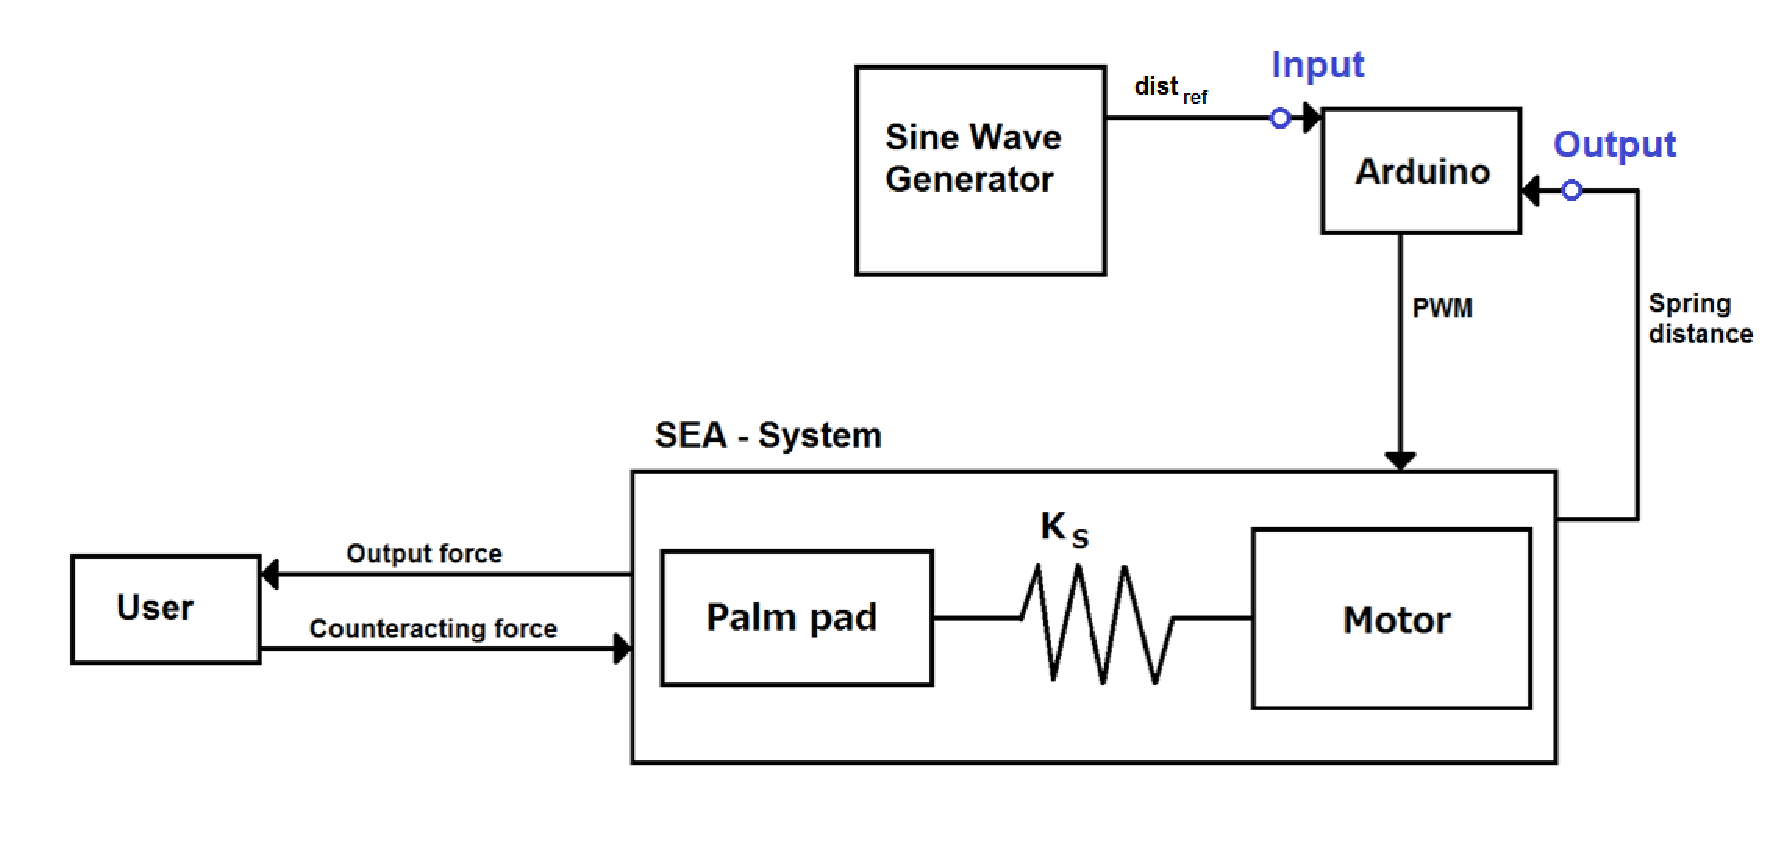
\includegraphics[width=0.6\linewidth]{Figs/frf_measure_points}
		\caption{Control scheme for the frequency response analysis.}
		\label{fig:frf_measure_points}
	\end{figure}
	In this case the counteracting force from the user is infinite, since the palm pads have been blocked by a wall.
	
	\subsection{Photoreceptor Circuit}
	The circuit of the photoreceptor can be found in figure \ref{fig:tpr105_circuit}. The components chosen are the TPR-105 for the sensor, $R_1 = 330\Omega$ and $R_2 = 27k\Omega$.
	
	\begin{figure}[h!]
		\centering
		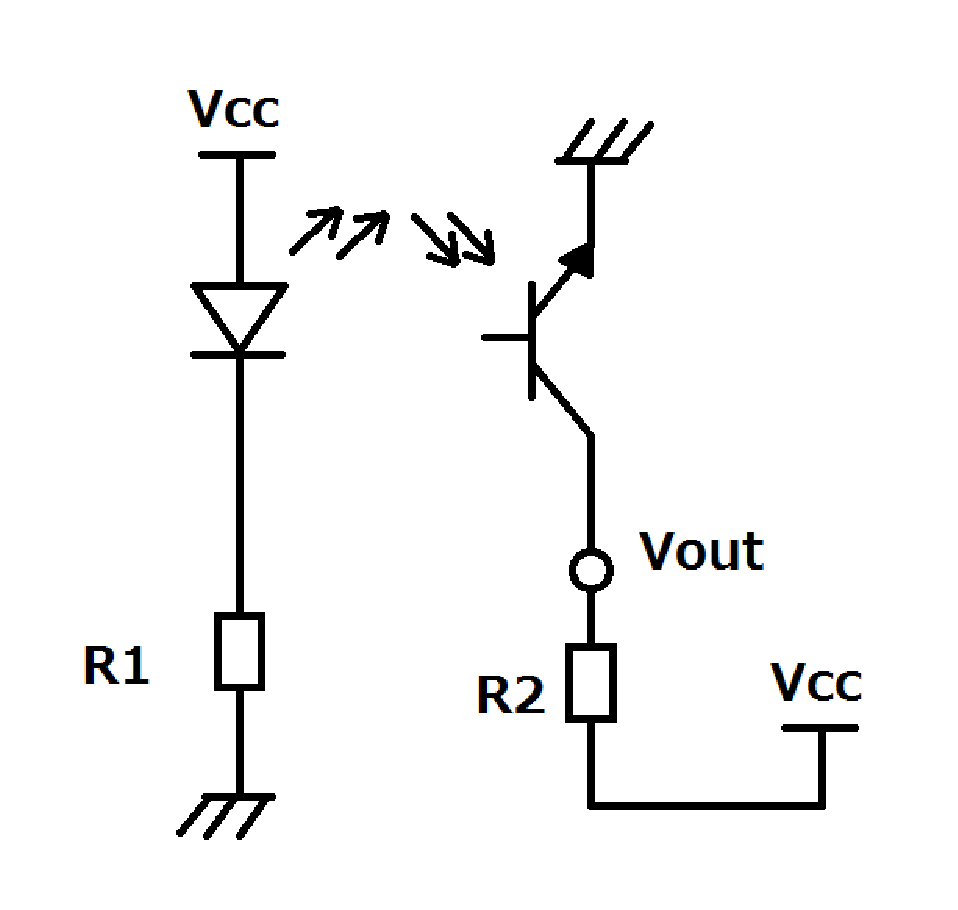
\includegraphics[width=0.2\linewidth]{Figs/tpr105_circuit}
		\caption{Photoreceptor circuit.}
		\label{fig:tpr105_circuit}
	\end{figure}
	The photoreceptors working principle is based on detecting the amount of reflected light. This controls the base current $i_B$ of the transistor in the schematic. This base current then determines the collector current $i_C$. Specific to this setup, the distance and therefore the output force controls the amount of light that is reflected on the wall of the palm pad. Therefore, we have:
	\begin{equation}
	F_{output} = k_{eq} \Delta x \propto i_B
	\end{equation}
	\begin{equation}
	i_C = h_{FE} i_B
	\end{equation}
	\begin{equation}
	V_{out} = V_{CC} - h_{FE} R_2 i_B = V_{CC} - K R_2 \Delta x
	\end{equation}
	Where $h_{FE}$ is the forward current gain and $K$ is a constant given by $h_{FE} k_{eq}$.
	
	The two resistor values have been empirically found to have the highest sensitivity but not saturating the measurement. The sensitivity decreases with a smaller resistor, since at a certain point, the Arduino cannot detect a change in voltage anymore. Saturation occurs, when the value of $R_2$ is too high.
	
	\subsection{Identification of Operational Range (Photoreceptor)}
	To find the receptor values at maximum compression of the springs, a simple test has been made, where one time $0$V has been applied to the motors, and another time $20$V has been applied. This $20$V value is within a safety margin of the maximum applicable voltage given by the datasheet of the motors. The result can be seen in figure \ref{fig:max_volt_applied_plot}.
	
	\begin{figure}[h!]
		\centering
		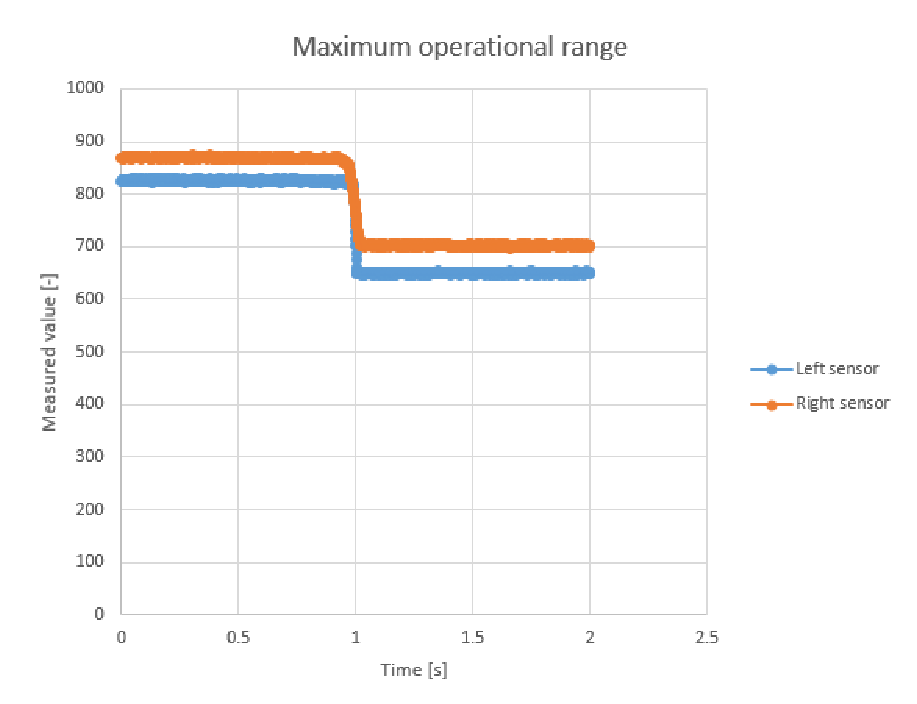
\includegraphics[width=0.6\linewidth]{Figs/max_volt_applied_plot}
		\caption{Operational range of photoreceptor with springs at rest and in full compression.}
		\label{fig:max_volt_applied_plot}
	\end{figure}
	
	The values that have been found to be the limiting values are resumed in table \ref{tab:oper_range_PS}.
	
	\begin{figure}[h!]
		\centering
		\begin{tabular}{|l|c|c|c|c|c|}
			\hline
			& Sensor reading & Distance & Sensor reading & Distance & Max output  \\
			& MAX (rest) & (rest) & MIN (compression) & (compression) & force \\ \hline \hline
			Left side & 830 & 2.35mm & 650 & 4mm & 9.9N \\ \hline
			Right side & 870 &2.2mm & 700 & 4mm & 10.8N \\ \hline
		\end{tabular}
		\caption{Identified operational range for the photoreceptors in the PlayStation controller.}
		\label{tab:oper_range_PS}
	\end{figure}
	
	Using these values, the photoreceptor measurements can be mapped to this range with an 8-bit value. This means that $0$ is no compression and $255$ is fully achievable compression.
	
	\section{Frequency Response Analysis}
	To conduct the frequency response analysis in a meaningful environment, the controller has to be tested under conditions close to the operational ones. To be able to control the distance between the palm pads and the L-plates, and therefore the compression ratio of the springs, the palm pads have been blocked mechanically. With the wave generator producing the reference signal, the Arduino controlled the motors to match the compression with the reference. Figures \ref{fig:1plot_zoom} to \ref{fig:100plot_zoom} show some testcases.
	
	
	\begin{figure}[!htb]
		\minipage{0.32\textwidth}
		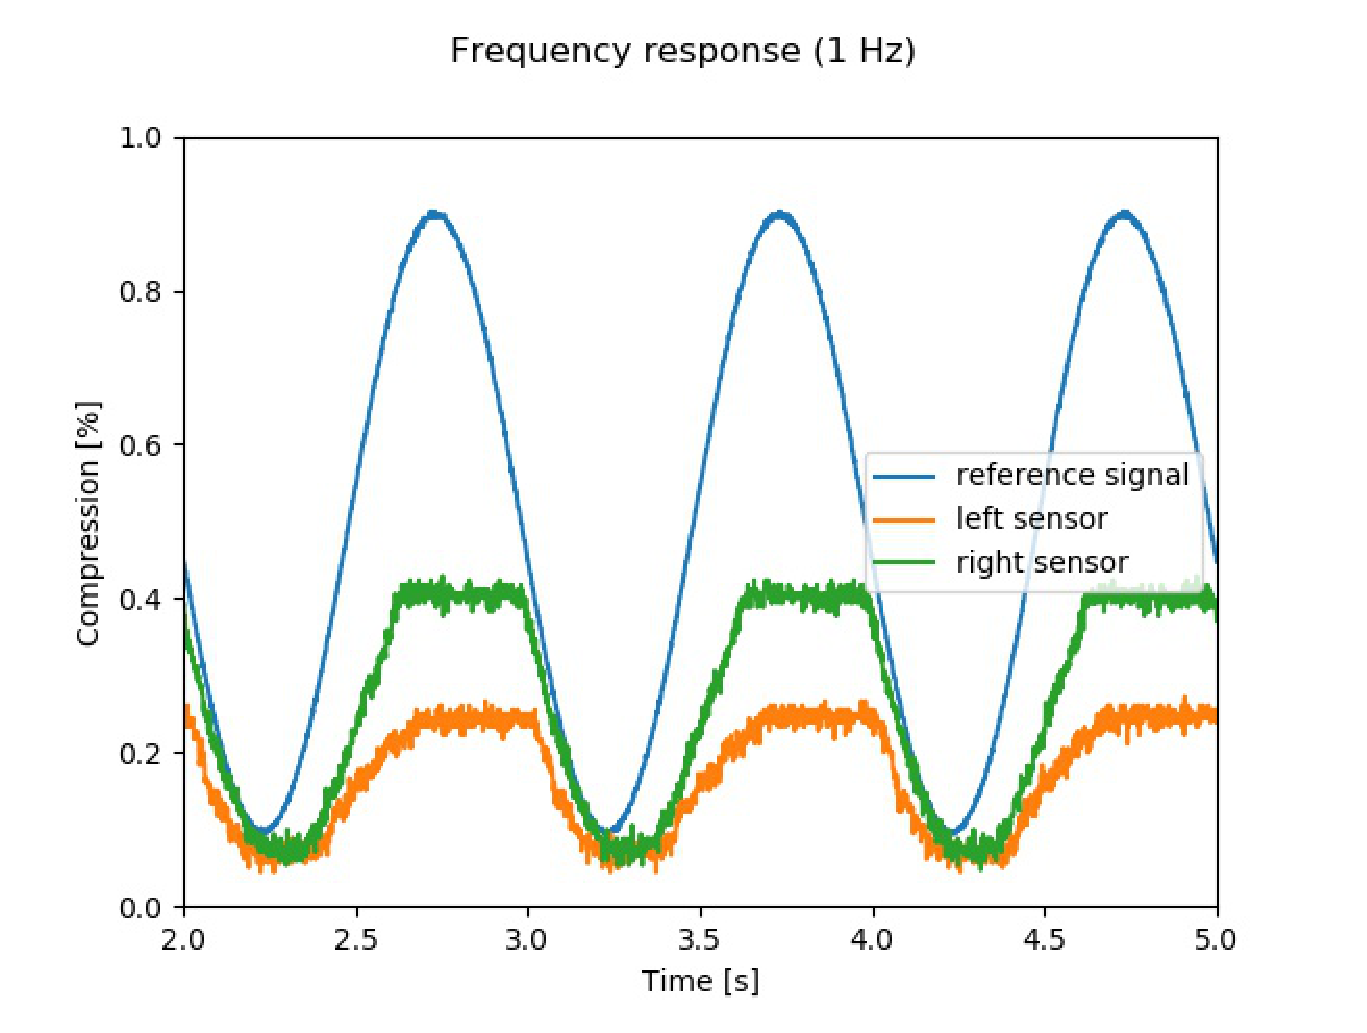
\includegraphics[width=\linewidth]{Figs/1plot_zoom}
		\caption{1 Hertz}\label{fig:1plot_zoom}
		\endminipage\hfill
		\minipage{0.32\textwidth}
		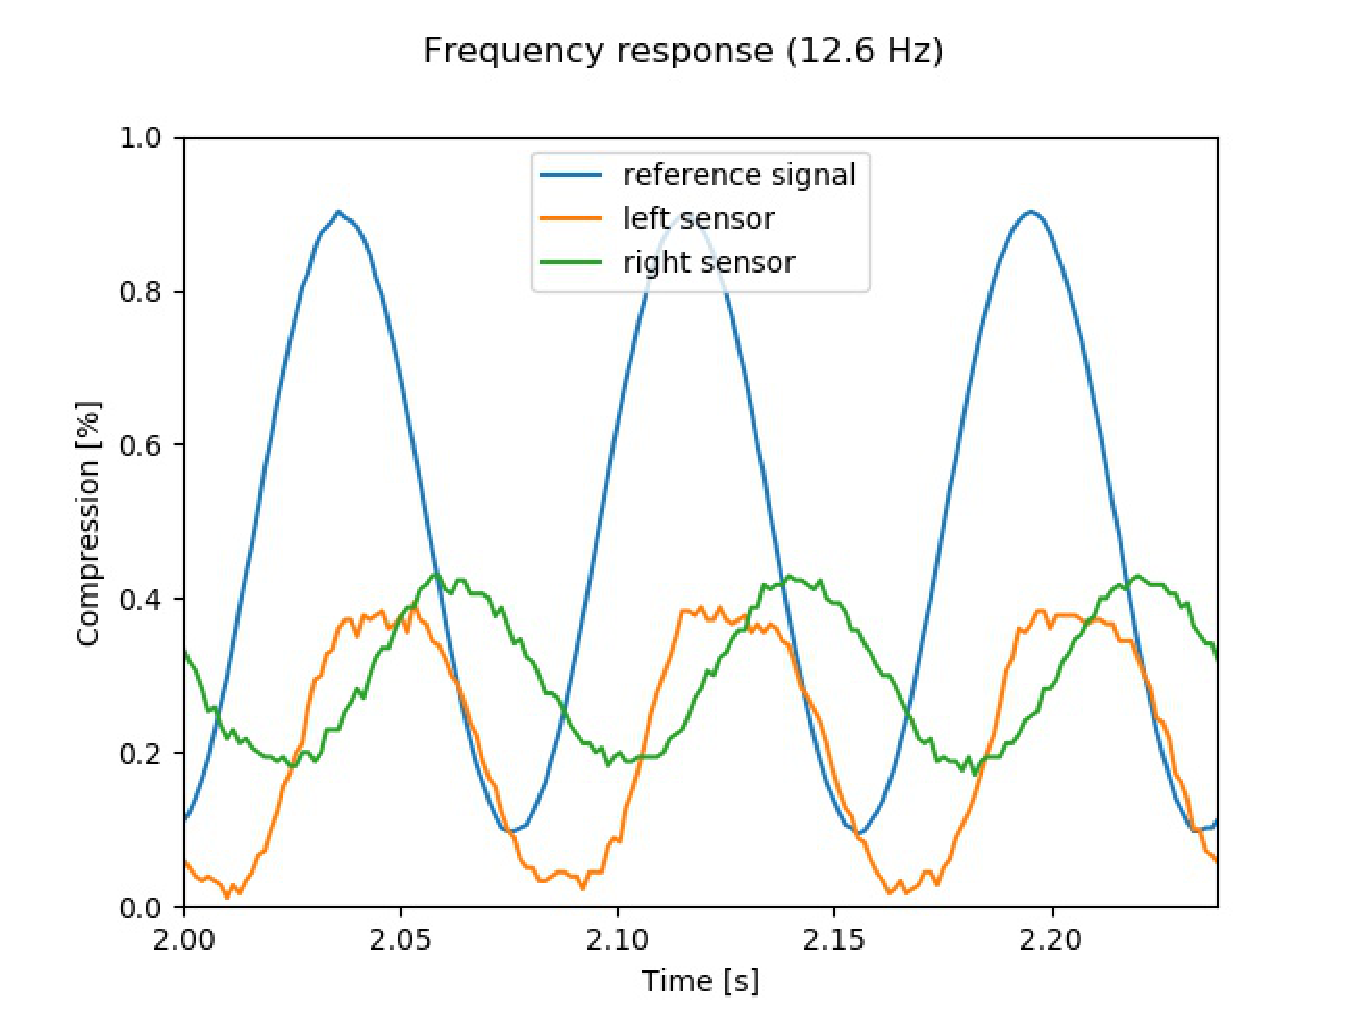
\includegraphics[width=\linewidth]{Figs/12.6plot_zoom.eps}
		\caption{12.6 Hertz}\label{fig:12.6plot_zoom}
		\endminipage\hfill
		\minipage{0.32\textwidth}%
		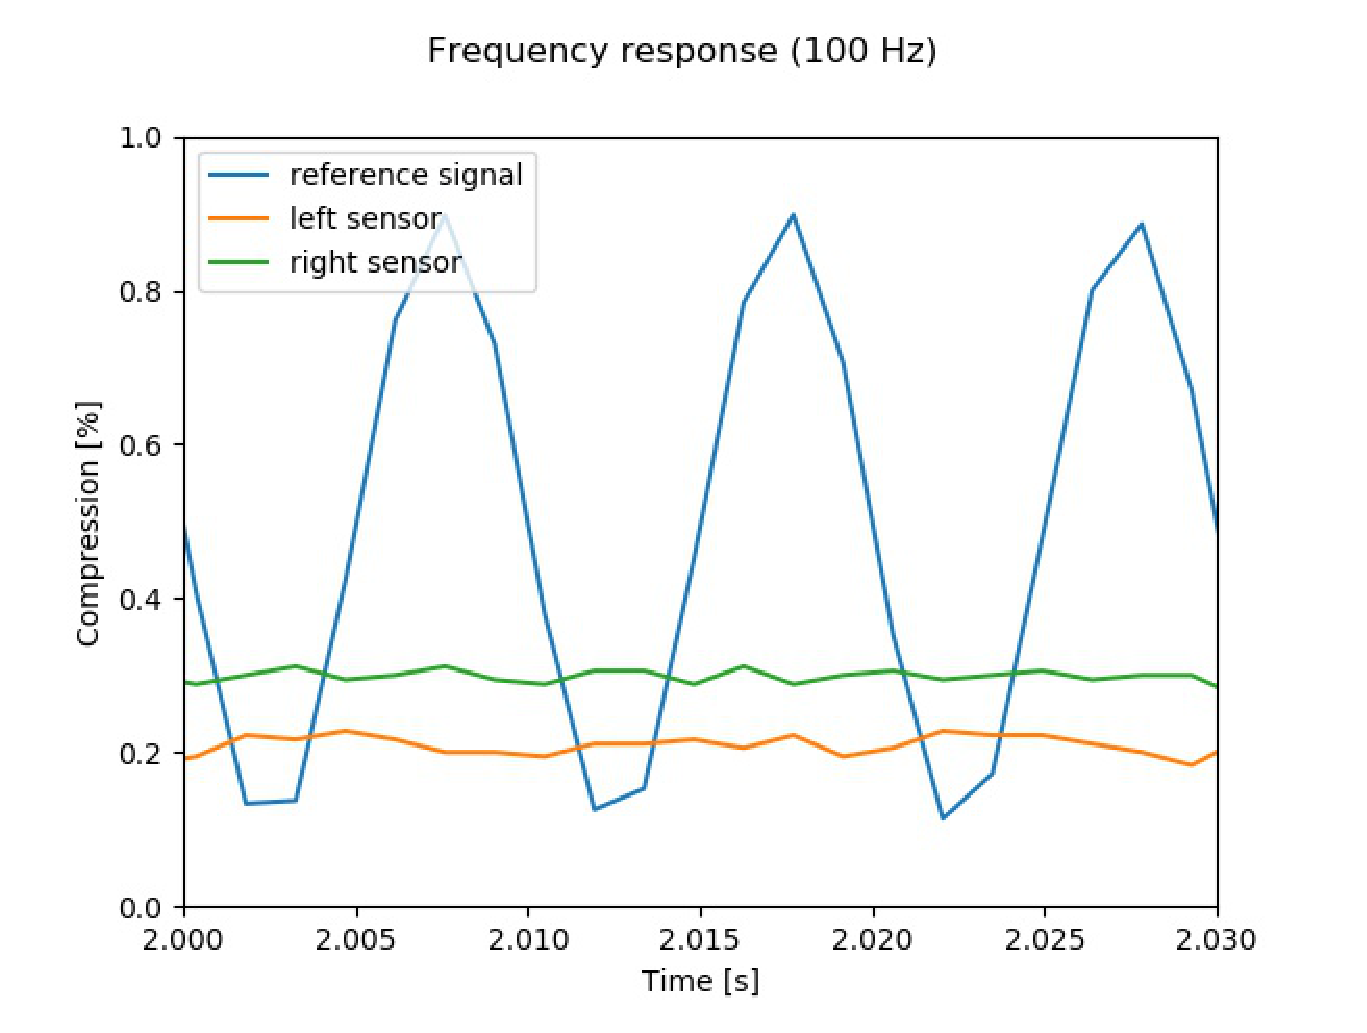
\includegraphics[width=\linewidth]{Figs/100plot_zoom}
		\caption{100 Hertz}\label{fig:100plot_zoom}
		\endminipage
	\end{figure}
	With these signals one can calculate the amplification factor between the reference signal and the output signal, as well as the phase shift.
	
	
	\subsection{Sinewave Fitting}
	As described in this example\cite{exnumerus2010}, one can fit a sinewave with the linear least square method to the samples. For finding the amplitude the second norm%TODO why not RMS as explained in slides_frf_and_bode_plots.pdf
	 has been used. This function returns the phase, amplitude and the bias. In this case, the difference in phase between input and output, as well as the amplitude ratio is needed in order to plot a Bode diagram.
	
	\subsection{Bode Diagram}
	The results of the frequency response analysis are shown in figures \ref{fig:bode_left} and \ref{fig:bode_right}.
	
	\begin{figure}[!htb]
		\minipage{0.48\textwidth}
		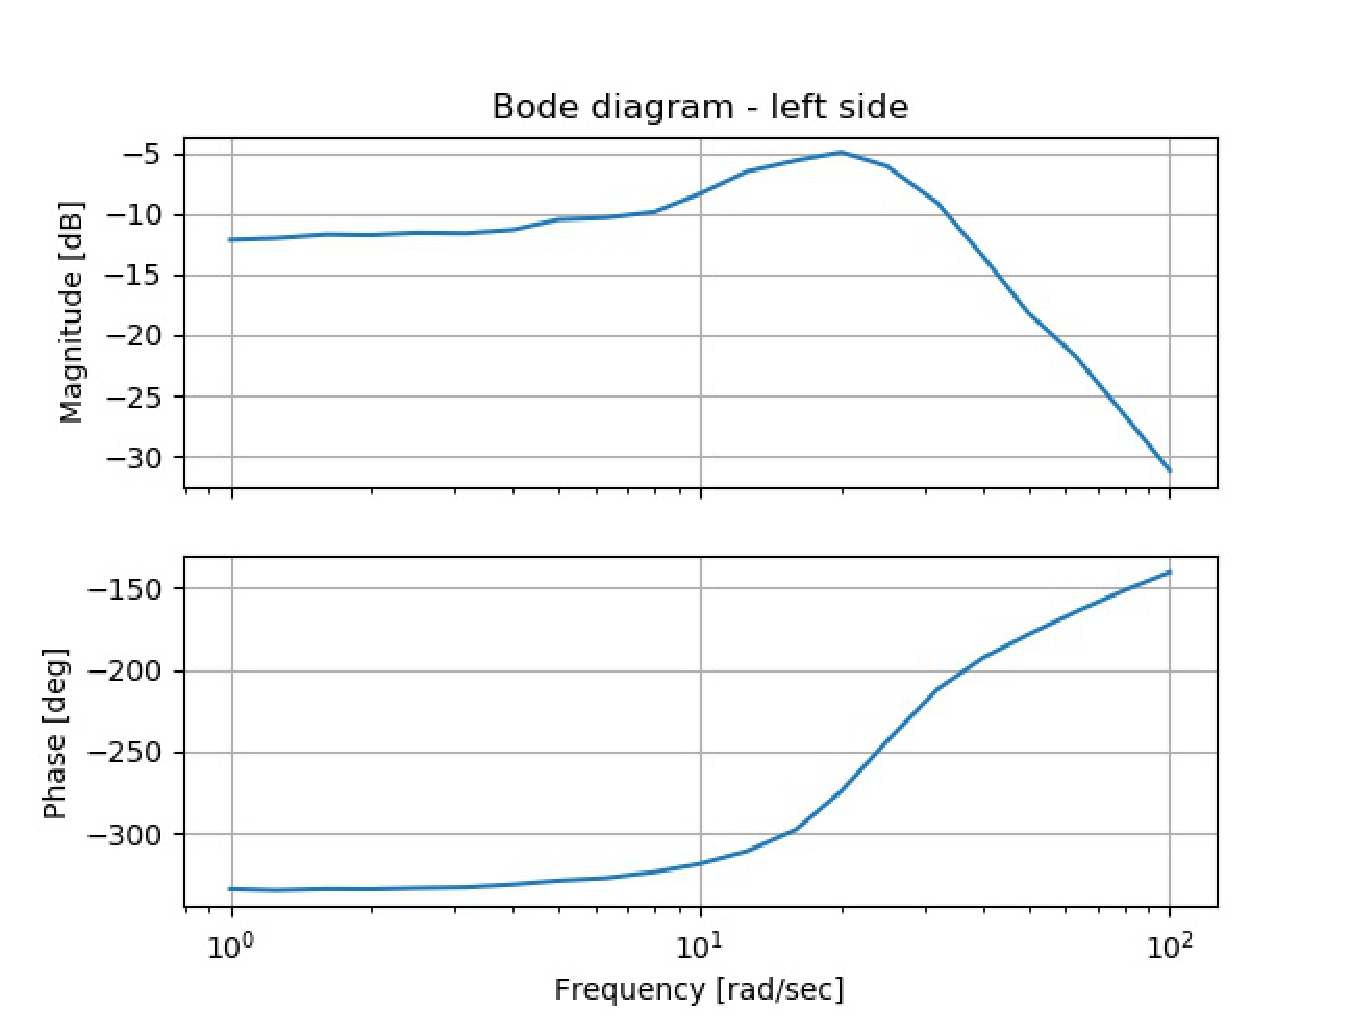
\includegraphics[width=\linewidth]{Figs/bode_left}
		\caption{Left-hand side, Motor reduction ratio $33:1$}\label{fig:bode_left}
		\endminipage\hfill
		\minipage{0.48\textwidth}
		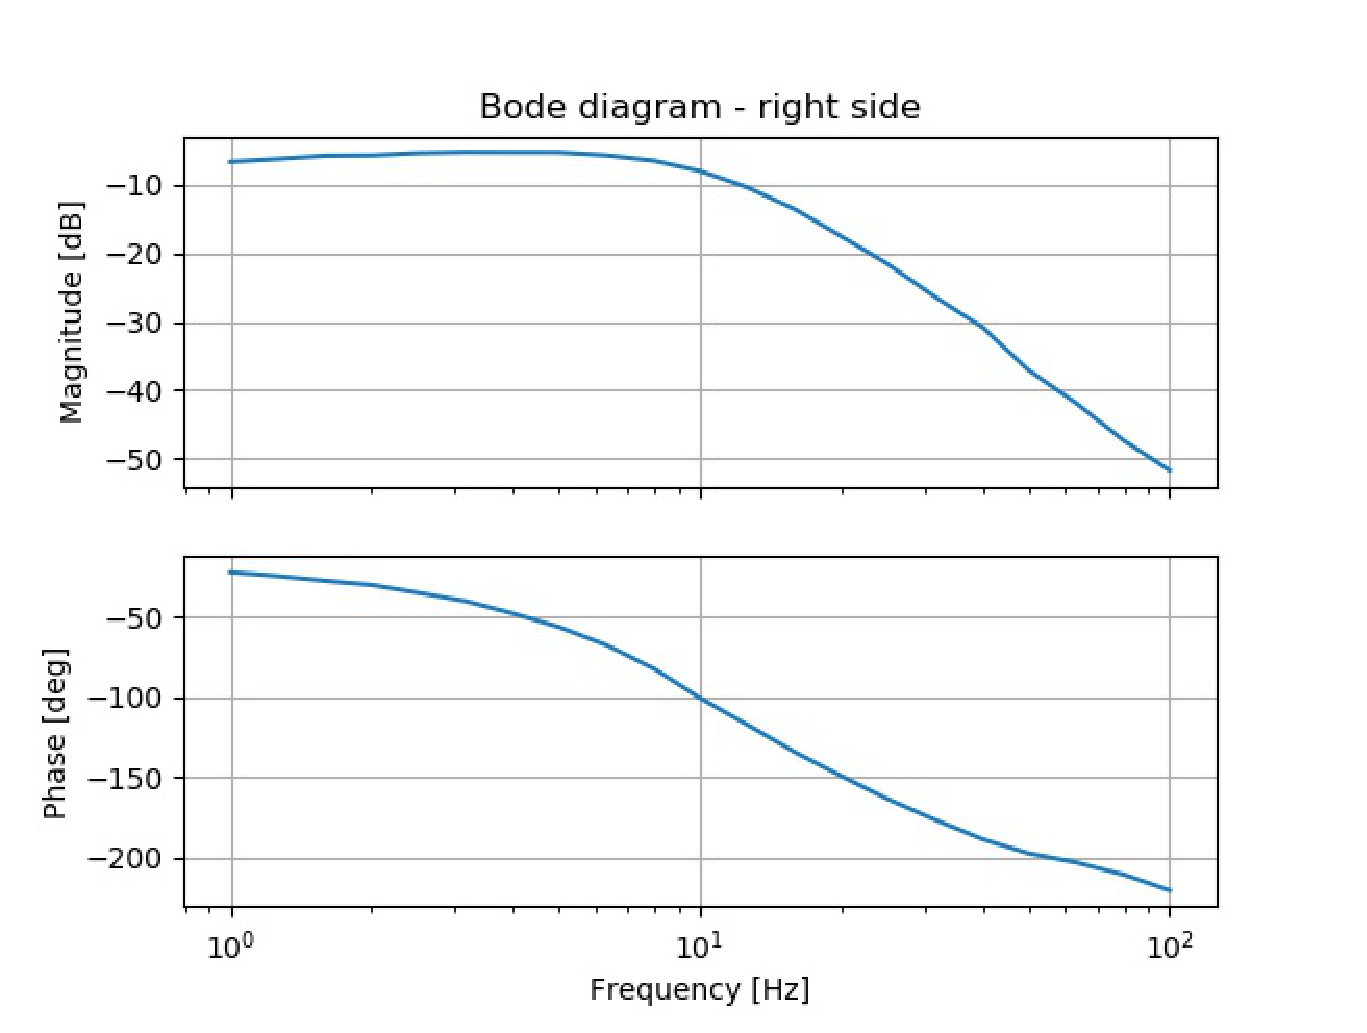
\includegraphics[width=\linewidth]{Figs/bode_right}
		\caption{Right-hand side, Motor reduction ratio $112:1$}\label{fig:bode_right}
		\endminipage\hfill
	\end{figure}

	For the left-hand side, a resonance top at around $13$Hz can be found, with a gain of roughly $-12$dB for lower frequencies. At higher frequencies a slope of roughly $-26$dB/dec has been calculated. For doing so the values in the range of $50$Hz and $100$Hz have been used. The phase shifts from $-25^\circ$ to $-222^\circ$, a total shift of roughly $200^\circ$.\\
	For the right-hand side, no resonance top is visible, and a constant gain of roughly $-6$dB for lower frequencies can be identified. At higher frequencies a slope of roughly $-30$dB/dec has been calculated. Again using the values in the range of $50$Hz and $100$Hz. The phase shifts from $-25^\circ$ to $-223^\circ$, a total shift of roughly $200^\circ$.
	%in slides_frf_and_bode_plots.pdf slide 27 suggests that the pole is stable since it goes from 0 to -180
	
	\section{Discussion}
	As it can be seen in figues \ref{fig:1plot_zoom} to \ref{fig:100plot_zoom} the signal is not followed very smoothly. For one, the magnitude ratio even at low frequencies is at roughly $0.5$. This shows that the proportional gain is too low. This would not only lift up the curve indicated in the Bode diagram and shift it towards higher frequencies (to the right). Another important aspect is the saturation behavior of the right motor. The origin of this effect  needs to be investigated in more detail.\\
	From the Bode diagrams one can conclude several things. First of all, the gain magnitude at lower frequencies should be around $0$dB to have perfect following of the reference signal. This can be influenced by tuning the proportional value of the controller.\\
	Second, the two motors show different characteristics. While the weaker motor (left-hand side) shows a resonance top around $13$ Herz, the stronger motor has no such behavior. In order to have a more linear system, it is therefore favorable to use the stronger motor for this spring system.\\
	Furthermore, the first pole of the system can be found around $13$ Herz. The communication frequency between robot and graphical user interface is suggested (according to the datasheet of the robot) to be between $1$Hz and $5$Hz. This shows that the series elastic actuator system as it is implemented in this experiment, is not the limiting factor in the robotic system.\\
	When one wants to determine the order of the system, one can look at the slope at the tail of the magnitude curve in the Bode plot. In our case they are $-26$dB/dec and $-30$dB/dec for left and right respectively. Since the slopes can only be a multiple of $20$dB/dec, it can be concluded, that the $2 \xi \omega _0$ term from equation \ref{eq:transfer_fn_2nd_order} has a non-negligible influence at the tail of the Bode plot.
	The equation of a second order transfer function is as follows:
	\begin{equation}
		H (s) = \frac{\omega _0^2}{s^2 + 2 \xi \omega _0 s + \omega _0^2}
		\label{eq:transfer_fn_2nd_order}
	\end{equation}
	Therefore one should also have a look at the phase lag diagram. The phase shift of roughly $180^\circ$ suggests a second order transfer function.
	
	The only thing that might risk the reliability of the Bode diagrams is the fact that the output signal has shown to be electrically interfering with the input signal. This most probably comes from the fact that the output impedance is too high.

	\section{Conclusion}
	The Bode diagrams show promising results. This is a first hint that the implementation of the series elastic actuators is not slowing down the system, since the bottleneck is given by the robot GUI communication link.\\
	
	\section{Outlook}
	The input signal is interfering with the output signal on the Arduino. Therefore it is necessary to investigate its impact by implementing a voltage follower to reduce the output impedance.\\
	A theoretical model shall be calculated to take into account the different aspects and parameters of the setup. The goal is to come up with a precise model to simulate different parameter settings, such as equivalent spring constant, motor parameters or operating frequency.
	

	
	%�����܂�
}


